%%
%% This is file `mcmthesis-demo.tex',
%% generated with the docstrip utility.
%%
%% The original source files were:
%%
%% mcmthesis.dtx  (with options: `demo')
%% !Mode:: "TeX:UTF-8"
%% -----------------------------------
%%
%% This is a generated file.
%%
%% Copyright (C)
%%     2010 -- 2015 by latexstudio
%%     2014 -- 2016 by Liam Huang
%%
%% This work may be distributed and/or modified under the
%% conditions of the LaTeX Project Public License, either version 1.3
%% of this license or (at your option) any later version.
%% The latest version of this license is in
%%   http://www.latex-project.org/lppl.txt
%% and version 1.3 or later is part of all distributions of LaTeX
%% version 2005/12/01 or later.
%%
%% This work has the LPPL maintenance status `maintained'.
%%
%% The Current Maintainer of this work is Liam Huang.
%%
\documentclass{mcmthesis}
\mcmsetup{CTeX = true,   % 使用 CTeX 套装时,设置为 true
        tcn = 0123, problem = E,
        sheet = true, titleinsheet = true, keywordsinsheet = true,
        titlepage = true, abstract = false}
\usepackage{palatino}
\usepackage{lipsum}
\title{ Template for MCM Version \MCMversion}
\author{\small \href{http://www.latexstudio.net/}
  {
\includegraphics[width=7cm]{mcmthesis-logo}}}
 \setlength{\parindent}{2em} 
\date{\today}
\begin{document}
\begin{abstract}
 aaaaaaaa fffffffffffffffff ffffffffff ffffgggggggg gggggggggggggggggggggggggggg ggggggggggggggggg
i really really really want m prize meritable meri\par f
iiiiiii crazy
\begin{keywords}
Complex network;shortest path
\end{keywords}
\end{abstract}
\maketitle
\tableofcontents
\section{Introduction}
\subsection{Background}
\begin{itemize}
\item The evolutionary trajectory and intrinsic interactions of western popular music
\end {itemize}\quad
Nowadays, it has become a more and more common phenomenon for people to listen to all kinds of music to seek pleasure and relax themselves. And we may abstract and conclude the invariable key elements in the forever-changeable styles and contents of music. That are melody, harmony, lyrics, rhythm, and timbre, etc. And in analysing the similarity and developmental portraits among some of these elements, we may have a primary clue on how the previous musicians have exerted their influence upon their same and subsequent generations of musicians and give some insights into how a new genre of music came into being.\par
Utilizing the interactive network model, we are able to implement the cross-tabulation of the various specimens given, and further explore the deep-rooted relationship between different musicians over time, therefore produce a elementary work on the evolutionary trajectory of music.

\subsection{Restatement of the problem}\quad
From the data we retrieved.\cite{1} We can learn that all the artist in the world has their influences. Not only to the genre of music he specialized. But also to some specific artists from the younger generation. Our first mission is to create a network that links the influencer and the follower. Through the network,we may find the indicators of "musical influence". The weight and the form of the network can show us the relationship between different artists. They may be influencers, or followers. Or they can be both.\par
Similarity is also an index we focus to. Since there are experts already defined some features and factors of musical compositions. Features such as danceability, energy or liveness is hard to define by amateurs like us. However, the expert quantized these features so we can process them easily. In this case, we should find out that the similarity between artists from the same genre or from different genres.\par
The revolution of music through a period of time is also an significant argument we are facing. Each artists is active in different eras. Thus only the artists who became active earlier can influence the latter artists. Each era has their favorites, how does people's taste varies is also an interesting problem to solve.\par
Our model is meant to figure out the intrinsic information from the data we already knew. By processing the data with our model,we can learn a lot of hidden information. Hence we can answer the questions like: who is the major influencer of an era and how he led the popularity, which genre of music is the most popular one, how does the fashion changes over time. At last, we may even find out which genre will lead the major revolution of music.
\subsection{notation}
\begin{table}[]
\begin{tabular}{l|l}
ESV & Ecosystem service value                                   \\ \hline
DV  & Project caused decreased value                            \\
Ak  & Area of ecosystem k                                       \\
VCk & Ecological value coefficient per unit area of ecosystem k
\end{tabular}
\end{table}
\begin{itemize}%%前面加点的句子
\item minimizes the discomfort to the hands, or
\item maximizes the outgoing velocity of the ball.
\end{itemize}
We focus exclusively on the second definition.

\begin{itemize}
\item the initial velocity and rotation of the ball,
\item the initial velocity and rotation of the bat,
\item the relative position and orientation of the bat and ball, and
\item the force over time that the hitter hands applies on the handle.
\end{itemize}
\lipsum[3]
\begin{itemize}
\item the angular velocity of the bat,
\item the velocity of the ball, and
\item the position of impact along the bat.
\end{itemize}
\lipsum[4]
\emph{center of percussion} [Brody 1986], \lipsum[5]

\begin{Theorem} \label{thm:latex}
\LaTeX \quad 666
\end{Theorem}
\begin{Lemma} 
TeX .
\end{Lemma}
\begin{proof}
The proof of theorem.
\end{proof}

\subsection{Assumptions}
\lipsum[6]
\begin{itemize}
\item
\item
\item
\item
\end{itemize}

\lipsum[7]

\section{Analysis of the Problem}
\begin{figure}[h]%%插入图片
\small%%小图
\centering%%居中
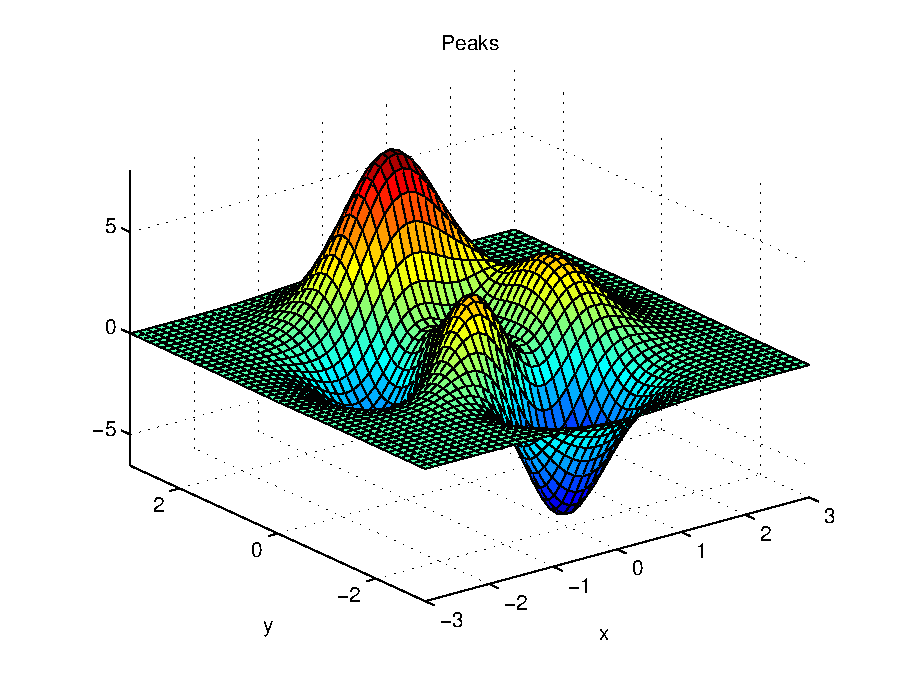
\includegraphics[width=12cm]{mcmthesis-aaa.eps}
\caption{aa} \label{fig:aa}
\end{figure}

\lipsum[8] \eqref{aa}
\begin{equation}
a^2 \label{aa}
\end{equation}


\begin{equation}
\frac{{w_{j}}^{(1)}{{w_{j}}^{(2)}{}}}{\sum_{j=1}^{n}{w_{j}}^{(1)}{w_{j}}^{(2)}}
\end{equation}
\[%%\[是不带编号的行间公式
  \begin{pmatrix}
  {a_{11} } & {a_{12} } & {a_{13} }  \\
  {a_{21} } & {a_{22} } & {a_{23} }  \\
  {a_{31} } & {a_{32} } & {a_{33} }  \\
  \end{pmatrix}
  = \frac{{Opposite}}{{Hypotenuse}}\cos ^{ - 1} \theta \arcsin \theta
\]
\lipsum[9]

\[
  p_{j}=\begin{cases} 0,&\text{if $j$ is odd}\\%%大括号输入方程组cases
  r!\,(-1)^{j/2},&\text{if $j$ is even}
  \end{cases}
\]

\lipsum[10]

\[
  \arcsin \theta  =
  \mathop{{\int\!\!\!\!\!\int\!\!\!\!\!\int}\mkern-31.2mu
  \bigodot}\limits_\varphi
  {\mathop {\lim }\limits_{x \to \infty } \frac{{n!}}{{r!\left( {n - r}
  \right)!}}} \eqno (1)
\]

\section{Calculating and Simplifying the Model  }
\lipsum[11]

\section{The Model Results}
\lipsum[6]

\section{Validating the Model}
\lipsum[9]

\section{Conclusions}
\lipsum[6]

\section{A Summary}
\lipsum[6]

\section{Evaluate of the Model}

\section{Strengths and weaknesses}
\lipsum[12]

\subsection{Strengths}
\begin{itemize}
\item \textbf{Applies widely}
This  system can be used for many types of airplanes, and it also
solves the interference during  the procedure of the boarding
airplane,as described above we can get to the  optimization
boarding time.We also know that all the service is automate.
\item \textbf{Improve the quality of the airport service}\\
Balancing the cost of the cost and the benefit, it will bring in
more convenient  for airport and passengers.It also saves many
human resources for the airline. \item \textbf{}
\end{itemize}

\begin{thebibliography}{99}%%跳出reference 写引用文献
\bibitem{1} D.~E. KNUTH   The book  the American
Mathematical Society and Addison-Wesley
Publishing Company , 1984-1986.
\bibitem{2}Lamport, Leslie,  : `` A Document Preparation System '',
Addison-Wesley Publishing Company, 1986.
\bibitem{3}\url{http://www.latexstudio.net/}
\bibitem{4}\url{http://www.chinatex.org/}
\end{thebibliography}

\begin{appendices}

\section{First appendix}

\lipsum[13]

Here are simulation programmes we used in our model as follow.\\

\textbf{\textcolor[rgb]{0.98,0.00,0.00}{Input matlab source:}}
\lstinputlisting[language=Matlab]{./code/mcmthesis-matlab1.m}

\section{Second appendix}

some more text \textcolor[rgb]{0.98,0.00,0.00}{\textbf{Input C++ source:}}
\lstinputlisting[language=C++]{./code/mcmthesis-sudoku.cpp}

\end{appendices}
\end{document}

%%
%% This work consists of these files mcmthesis.dtx,
%%                                   figures/ and
%%                                   code/,
%% and the derived files             mcmthesis.cls,
%%                                   mcmthesis-demo.tex,
%%                                   README,
%%                                   LICENSE,
%%                                   mcmthesis.pdf and
%%                                   mcmthesis-demo.pdf.
%%
%% End of file `mcmthesis-demo.tex'.
